\documentclass[11pt]{article}
\usepackage[pdftex]{graphicx}
\usepackage{amsmath}
\usepackage{amssymb}
\usepackage[numbers]{natbib}
\usepackage{hyperref}

\DeclareGraphicsRule{.tif}{png}{.png}{`convert #1 `dirname #1`/`basename #1 .tif`.png}

\newcommand{\com}[1]{\textbf{#1}}
\newcommand{\inparam}{$\Leftarrow$}
\newcommand{\outparam}{$\Rightarrow$}

\newcommand{\commandcolumna}{0.11\textwidth}
\newcommand{\commandcolumnb}{0.22\textwidth}
\newcommand{\commandcolumnc}{0.60\textwidth}

\hypersetup{
    bookmarks=true,
    unicode=false,
    pdftoolbar=true,
    pdfmenubar=true,
    pdffitwindow=false,
    pdfstartview={FitH},
    pdftitle={The Woolz Internet Image Protocol (IIP) Server (Version 1.1.6)},
    pdfauthor={Bill Hill},
    pdfsubject={Woolz Internet Image Protocol Server},
    pdfcreator={Bill Hill},
    pdfproducer={MRC HGU at the IGMM, University of Edinburgh},
    pdfkeywords={image server} {3d image},
    colorlinks=true,
    linkcolor=blue,
    citecolor=blue,
    filecolor=magenta,
    urlcolor=red
}

\newfont{\sltt}{cmsltt10}  % font for command argument (slanted typewriter)

\title{The Woolz Internet Image Protocol (IIP) Server (Version 1.1.6)}
\author{
  Zsult Husz \footnote{Supported by {NIH} under grant \#1R01MH070370-01A2.} \\
  \and
  Bill Hill \footnote{bill.hill@igmm.ed.ac.uk}
}

\begin{document}

\pagenumbering{roman}
\addcontentsline{toc}{section}{Title Page}
\maketitle

\begin{abstract}
The Woolz Internet Imaging Protocol (IIP) server (WlzIIPSrv) extends
the {IIP} to allow views of 3D Woolz objects with multiple components.
This manual describes these extensions for both users and developers
of the WlzIIPSrv.
\end{abstract}

\addcontentsline{toc}{section}{Abstract}

\newpage

\tableofcontents
\addcontentsline{toc}{section}{Contents}

\newpage

\pagenumbering{arabic}

\section{Introduction}

The Internet Imaging Protocol {IIP} provides quick access to large image
databases allowing large images to be viewed remotely. It makes use of
tile-based delivery so that panning and zooming within large images
is  possible without needing to download the entire image.
The computational requirements of the client machine for viewing are low,
allowing viewers to be implemented within web browsers.
However, it is limited to 2D images.
In biomedical imaging (and many other fields) {3D} images are routinely used.
A set of extensions to the {IIP} server was developed within the Edinburgh
Mouse Atlas Project \cite{EMAP} to allow the remote visualization of sections
through large 3D objects.
These extensions make use of many of the features of Woolz, an image
processing system with it's own efficient image representation \cite{WOOLZ}.

This document assumes understanding of the IIP \citep{IIP97}.

For clarity, in the rest of this document IIPSrv will refer to the original
{IIP}  server, with code version 0.9.7 \citep{IIPSRV097}, WlzIIPSrv will refer
to the extended server, while IIP will point to the protocol standard of
\cite{IIP97}.

The coordinate system convention used in this document is shown in
Figure~\ref{fig:coordinates}.
The object coordinate is defined by the object and the section coordinates
result after sectioning. Then, the translated section coordinates with the
section's minimum at $(0,0)$ are the display coordinates.
Further, the section is divided into non-overlapping tiles covering the
whole section.
Tiles are numbered with 0, 1, 2, etc., with the $0^{th}$ coordinates matching
the display coordinates.
The  and $1^{st}$,$2^{nd}$, etc. tiles continue from left to right and top to
bottom.
A client can visualise a section with reduced viewing area.
This has the view coordinates and is client dependent.
\begin{figure}[!htb]
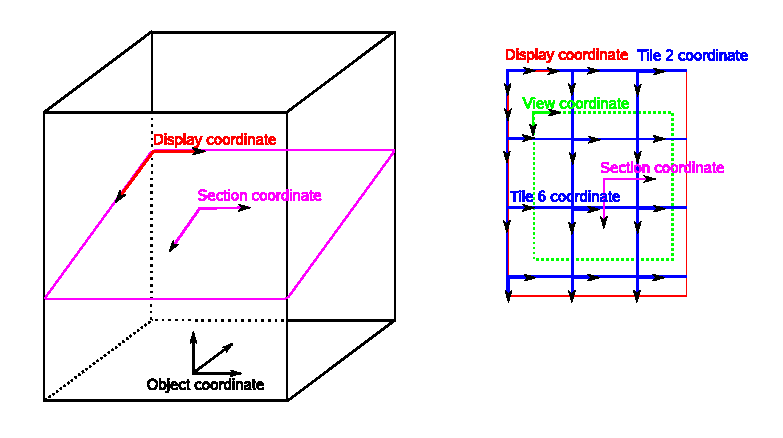
\includegraphics[width=\linewidth]{coordinates}
\caption{Coordinate systems}
\label{fig:coordinates}
\end{figure}

\section{Extension overview}

In addition to the IIPSrv commands, a WlzIIPSrv command specifies an object,
sets the viewing section parameters and requests  image or meta data of the
object.
Tile request are similar to the TIFF requests,
however for a Woolz object the resolution number used in \com{JTL/TIL} is
ignored.

%TODO: Some of original IIP commands are incompatible with the new Woolz
%      commands.

The extended command list that sets query parameters are summarised in
Table~\ref{tab:commands}, while Table~\ref{tab:objects} shows the new objects
that may be queried with the \com{OBJ} command.

\begin{table}[!hp]
\begin{tabular}{|p{0.15\textwidth}|p{0.5\textwidth}|p{0.45\textwidth}|}
\hline
\textbf{Command} &  \textbf{Purpose} & \textbf{Syntax}\\
\hline
\com{CVT} & Request an image to be returned as a composed image. CVT accepts now also PNG and WLZ format requests.& \texttt{CVT={\sltt format}}\\
\com{DST} & Specify the distance of the sectioning plane& \texttt{DST={\sltt dis}}\\
\com{FXP} & Specify the fixed point of the viewing section rotation & \texttt{FXP={\sltt X,Y,Z}}\\
\com{FXT} & Specify the second fixed point of the viewing section rotation & \texttt{FXT={\sltt X,Y,Z}}\\
\com{MAP} & Define a colour or grey value mapping & \texttt{MAP=
                                    \newline
                                    {\sltt mspec[,mspec[,mspec[,mspec]]]}}
                                    \newline
				    where
				    {\sltt mspec}={\sltt t,il,iu,ol,ou,p0,p1} \\
\com{MOD} & Specify the projection mode & \texttt{MOD={\sltt mode}} \\
\com{PAB} & Specify the 3D query point absolute in the object coordinate& \texttt{PAB={\sltt X,Y,Z}}\\
\com{PIT} & Specify the pitch angle of the sectioning rotation& \texttt{PIT={\sltt angle}}\\
\com{PRL} & Specify the 2D query point relative in tile or display or tile coordinate& \texttt{PRL={\sltt T,X,Y}}\\
\com{PTL} & Retrieve a tile as a PNG image& \texttt{PTL={\sltt res,tile}}\\
\com{DPT} & Specify the rendering depth & \texttt{DPT={\sltt depth}} \\
\com{RMD} & Specify the rendering mode & \texttt{RMD={\sltt mode}} \\
\com{ROL} & Specify the roll angle of the sectioning rotation & \texttt{ROL={\sltt angle}}\\
\com{SCL} & Specify the scale used in the sectioning transformation & \texttt{SCL={\sltt scale}} \\
\com{SEL} & Specify a component of a compound object to be displayed and its
colour. See \ref{ssec:imgpexp}. & \texttt{SEL={\sltt E,R,G,B,A}}\\
\com{UPV} & Specify the up vector for the \com{UP\_IS\_UP} mode & \texttt{UPV={\sltt X,Y,Z}}\\
\com{WLZ} & Specify the Woolz object & \texttt{WLZ={\sltt path}}\\
\com{YAW} & Specify the yaw angle of the sectioning rotation& \texttt{YAW={\sltt angle}} \\
\hline
\end{tabular}
\caption{Extended command overview}
\label{tab:commands}
\end{table}

\begin{table}[!hp]
\begin{tabular}{|p{0.25\textwidth}|p{0.75\textwidth}|}
\hline
\textbf{Object} &\textbf{Purpose}\\
\hline
\com{IIP-server}            & Identify if WLZ-IIP is running. \\
\com{Max-size}              & The size of the section. \\
\com{Tile-size}             & The size of a tile. \\
\com{Wlz-true-voxel-size}   & The voxel size of the object. \\
\com{Wlz-volume}            & The volume of the object or first selection (if it exists). \\
\com{Wlz-n-component}       & The number of components in a compound object. \\
\com{Wlz-distance-range}    & The range of the sectioning plane distance. \\
\com{Wlz-sectioning-angles} & The pitch, yaw and roll angles of of the sectioning plane. \\
\com{Wlz-coordinate-3D}     & The 3D coordinates defined in 2D by the \com{PRL} command. \\
\com{Wlz-grey-stats}        & Simple statistics of the image values of the object or first selection (if it exists). \\
\com{Wlz-grey-value}        & The grey or RGB value of a point specified either the \com{PRL} or the \com{PAB} commands. \\
\com{Wlz-transformed-coordinate-3d} & The display coordinates and displacement from the sectioning plane of a 3D point
                                      defined by \com{PAB}. \\
\com{Wlz-foreground-objects}& The components of the compound object that 2D/3D query point is a foreground. \\
\hline
\end{tabular}
\caption{Extended object overview}
\label{tab:objects}
\end{table}


\subsection{Woolz object specification}

\begin{tabular}{p{\commandcolumna}p{\commandcolumnb}p{\commandcolumnc}}
\com{WLZ} & \textbf{Purpose} &
Specify the Woolz object. It is similar to the \com{FIF} command, however instead of loading Pyramidal Tiled TIFF images, it specifies a Woolz object. Compered with \com{FIF}, the Woolz object is not loaded until a later operation requires this. The Woolz objects are cached.
3D domain and value objects, and compound objects with 3D domain or value components are supported. For a compound object the domain of the first object must
include all other object domains. If file name ends with \texttt{.gz}, gzipped Woolz object is expected.\\
& \textbf{Syntax} & \texttt{WLZ={\sltt path}}\\
& \textbf{Input Parameters}& \texttt{PATH {\sltt path}} Full path of the Woolz object.\\
& \textbf{Response} & \com{WLZ} returns nothing when accompanied by other commands\\
& \textbf{Example} & \outparam\texttt{WLZ=/home/bill/pics/lobster3d.wlz}\\
& \textbf{Notes} & Equivalent if \com{FIF} \citep[p.25]{IIP97}\\
\end{tabular}

\subsection{Setting sectioning and query parameters}

The following commands are optional and can be used in any combination.

\hrule\noindent
\begin{tabular}{p{\commandcolumna}p{\commandcolumnb}p{\commandcolumnc}}
\com{DST} & \textbf{Purpose} &
Specify the distance of the sectioning plane\\
& \textbf{Syntax} & \texttt{DST={\sltt dis}}\\
& \textbf{Input Parameters}& \texttt{FLOAT {\sltt dis}} \newline The distance to the sectioning plane\\
& \textbf{Response} & none\\
& \textbf{Example} & \outparam\texttt{DST=12.5}\\
& \textbf{Default value} & \texttt{0.0}\\
\end{tabular}
\hrule\noindent
\begin{tabular}{p{\commandcolumna}p{\commandcolumnb}p{\commandcolumnc}}
\com{FXP} & \textbf{Purpose} & 
Specify the view rotation fixed point in the object coordinate system.\\
& \textbf{Syntax} & \texttt{FXP={\sltt X,Y,Z}}\\
& \textbf{Input Parameters}& \texttt{FLOAT {\sltt X}} \newline The x coordinate\newline 
\texttt{FLOAT {\sltt Y}} \newline The y coordinate\newline
\texttt{FLOAT {\sltt Z}} \newline The z coordinate\\
& \textbf{Response} & none\\
& \textbf{Example} & \outparam\texttt{FXP=10.5,20,15.0}\\
& \textbf{Default value} & \texttt{0.0,0.0,0.0}\\
\end{tabular}
\hrule\noindent
\begin{tabular}{p{\commandcolumna}p{\commandcolumnb}p{\commandcolumnc}}
\com{FXT} & \textbf{Purpose} & 
Specify the second fixed point in the object coordinate system of the viewing section rotation used only with \texttt{MOD=FIXED\_LINE}.\\
& \textbf{Syntax} & \texttt{FXT={\sltt X,Y,Z}}\\
& \textbf{Input Parameters}& \texttt{FLOAT {\sltt X}} \newline The x coordinate\newline 
\texttt{FLOAT {\sltt Y}} \newline The y coordinate\newline
\texttt{FLOAT {\sltt Z}} \newline The z coordinate\\
& \textbf{Response} & none\\
& \textbf{Example} & \outparam\texttt{FXT=30,-20.2,15.0}\\
& \textbf{Default value} & \texttt{0.0,0.0,0.0}\\
\end{tabular}
\hrule\noindent
\begin{tabular}{p{\commandcolumna}p{\commandcolumnb}p{\commandcolumnc}}
\com{MAP} & \textbf{Purpose} &
Defines a colour or grey value mapping.
Grey values outside the mapped region are clamped to the minimum and maximum output colour componentor grey values.
There may be 1,2,3 or 4 mapping specifications given; with a single mapping specification meaning a grey value mapping,
two specifications a grey with alpha mapping, three an RGB mapping and four an RGB$\alpha$ mapping.\\
& \textbf{Syntax} & \texttt{MAP={\sltt mspec[,mspec[,mspec[,mspec]]]}}
                    \newline where {\sltt mspec}={\sltt t,il,iu,ol,ou,p0,p1} \\
& \textbf{Input Parameters}& \texttt{\sltt {t $\in$ IDENTITY | LINEAR | GAMMA | SIGMOID}} \newline The mapping function\newline
                             \texttt{FLOAT {\sltt il}} \newline Input lower grey value\newline
                             \texttt{FLOAT {\sltt il}} \newline Input upper grey value\newline
                             \texttt{FLOAT {\sltt ol}} \newline Output lower colour component or grey value\newline
                             \texttt{FLOAT {\sltt ol}} \newline Output upper colour component or grey value\newline
                             \texttt{FLOAT {\sltt p0}} \newline Gamma ($\gamma$)or first sigmoid parameter ($\mu$)\newline
                             \texttt{FLOAT {\sltt p1}} \newline Second sigmoid parameter ($\sigma$)\newline\\
& \textbf{Response} & none\\
& \textbf{Example} & \outparam\texttt{MAP=LINEAR,0,4095,0,255}\newline
                     Input grey values in the range 0-4095 are mapped to output values with the range 0-255\\
& \textbf{Default value} & \texttt{IDENTITY}\\
\end{tabular}
\hrule\noindent
\begin{tabular}{p{\commandcolumna}p{\commandcolumnb}p{\commandcolumnc}}
\com{MOD} & \textbf{Purpose} & Specify projection mode.\\
& \textbf{Syntax} & \texttt{MOD={\sltt mode}} \\
& \textbf{Input Parameters}& \texttt{{\sltt mode} $\in$ STATUE | UP\_IS\_UP | FIXED\_LINE | ZERO\_ZETA | ZETA} \newline The projection mode\\
& \textbf{Response} & none\\
& \textbf{Example} & \outparam\texttt{MOD=FIXED\_LINE}\\
& \textbf{Default value} & \texttt{UP\_IS\_UP}\\
\end{tabular}
\hrule\noindent
\begin{tabular}{p{\commandcolumna}p{\commandcolumnb}p{\commandcolumnc}}
\com{PIT} & \textbf{Purpose} &
Specify the pitch angle of the sectioning rotation\\
& \textbf{Syntax} & \texttt{PIT={\sltt angle}}\\
& \textbf{Input Parameters}& \texttt{FLOAT {\sltt angle}} rotation angle in degrees\\
& \textbf{Response} & none\\
& \textbf{Example} & \outparam\texttt{PIT=180.0}\\
& \textbf{Range} & \texttt{0.0-180.0}\\
& \textbf{Default value} & \texttt{0.0}\\
\end{tabular}
\hrule\noindent
\begin{tabular}{p{\commandcolumna}p{\commandcolumnb}p{\commandcolumnc}}
\com{PAB} & \textbf{Purpose} & 
Specify a 3D query point absolute in the object coordinate system.\\
& \textbf{Syntax} & \texttt{PAB={\sltt X,Y,Z}}\\
& \textbf{Input Parameters}& \texttt{FLOAT {\sltt X}} \newline The x coordinate \newline
\texttt{FLOAT {\sltt Y}} \newline The y coordinate\newline
\texttt{FLOAT {\sltt Z}} \newline The z coordinate\\
& \textbf{Notes} & If both \com{PRL} and \com{PAB} are specified then \com{PRL} has priority of feature queries\\
& \textbf{Response} & none\\
& \textbf{Example} & \outparam\texttt{PAB=200,-50,30}\\
\end{tabular}
\hrule\noindent
\begin{tabular}{p{\commandcolumna}p{\commandcolumnb}p{\commandcolumnc}}
\com{PRL} & \textbf{Purpose} & 
Specify a 2D query point relative to tile or display coordinate system.\\
& \textbf{Syntax} & \texttt{PRL={\sltt T,X,Y}}\\
& \textbf{Input Parameters}& \texttt{RANGE {\sltt T}} \newline The T tile number\newline 
\texttt{RANGE {\sltt X}} \newline The x coordinate\newline
\texttt{RANGE {\sltt Y}} \newline The y coordinate\\
& \textbf{Notes} & \com{PRL} either specified a coordinate in a given tile, or if the tile number \texttt{{\sltt T}=-1} then in the display coordinates\\
& \textbf{Response} & none\\
& \textbf{Range} & \texttt{{\sltt T}=-1 .. maxtile}\newline {\sltt X,Y} are limited to the tile or section size\\
& \textbf{Example} & \outparam\texttt{PRL=2,20,1}\\
& \textbf{Default value} & none \\
\end{tabular}
\hrule\noindent
\begin{tabular}{p{\commandcolumna}p{\commandcolumnb}p{\commandcolumnc}}
\com{DPT} & \textbf{Purpose} &
Specify the rendering depth\\
& \textbf{Syntax} & \texttt{DPT={\sltt depth}}\\
& \textbf{Input Parameters}& \texttt{FLOAT {\sltt depth}} rendering depth for projection rendering modes, depth zero implies no limit\\
& \textbf{Response} & none\\
& \textbf{Example} & \outparam\texttt{DPT=10}\\
& \textbf{Default value} & \texttt{0}\\
\end{tabular}
\hrule\noindent
\begin{tabular}{p{\commandcolumna}p{\commandcolumnb}p{\commandcolumnc}}
\com{RMD} & \textbf{Purpose} &
Specify the rendering mode\\
& \textbf{Syntax} & \texttt{RMD={\sltt mode}}\\
& \textbf{Input Parameters}& \texttt{{\sltt mode} $\in$ SECT | PRJN |
PRJD | PRJV} \newline The rendering mode\\
& \textbf{Response} & none\\
& \textbf{Example} & \outparam\texttt{RMD=PRJV}\\
& \textbf{Default value} & \texttt{SECT}\\
\end{tabular}
\hrule\noindent
\begin{tabular}{p{\commandcolumna}p{\commandcolumnb}p{\commandcolumnc}}
\com{ROL} & \textbf{Purpose} &
Specify the roll angle of the sectioning rotation\\
& \textbf{Syntax} & \texttt{ROL={\sltt angle}}\\
& \textbf{Input Parameters}& \texttt{FLOAT {\sltt angle}} rotation angle in degrees\\
& \textbf{Response} & none\\
& \textbf{Example} & \outparam\texttt{ROL=20.0}\\
& \textbf{Range} & \texttt{0.0-360.0}\\
& \textbf{Default value} & \texttt{0.0}\\
\end{tabular}
\hrule\noindent

\begin{tabular}{p{\commandcolumna}p{\commandcolumnb}p{\commandcolumnc}}
\com{SCL} & \textbf{Purpose} &
Specify the scale used in the sectioning transformation.\\
& \textbf{Syntax} & \texttt{SCL={\sltt scale}} \\
& \textbf{Input Parameters}& \texttt{FLOAT {\sltt scale}} the scale. A values over one is up, while lower than one is down-scaling.\\
& \textbf{Response} & none\\
& \textbf{Example} & \outparam\texttt{SCL=2.5}\\
& \textbf{Range} & positive\\
& \textbf{Default value} & \texttt{1.0}\\
\end{tabular}
\hrule\noindent
\begin{tabular}{p{\commandcolumna}p{\commandcolumnb}p{\commandcolumnc}}
\com{UPV} & \textbf{Purpose} & 
Specify the up vector for the \texttt{UP\_IS\_UP} mode.\\
& \textbf{Syntax} & \texttt{UPV={\sltt X,Y,Z}}\\
& \textbf{Input Parameters}& \texttt{FLOAT {\sltt X}} \newline The x component \newline 
\texttt{FLOAT {\sltt Y}} \newline The y component\newline
\texttt{FLOAT {\sltt Z}} \newline The z component\\
& \textbf{Response} & none\\
& \textbf{Example} & \outparam\texttt{UPV=0,-1,2}\\
& \textbf{Default value} & \texttt{0.0,0.0,-1.0}\\
\end{tabular}
\hrule\noindent
\begin{tabular}{p{\commandcolumna}p{\commandcolumnb}p{\commandcolumnc}}
\com{YAW} & \textbf{Purpose} &
Specify the yaw angle of the sectioning rotation. \\
& \textbf{Syntax} & \texttt{YAW={\sltt angle}} \\
& \textbf{Input Parameters}& \texttt{FLOAT {\sltt angle}} rotation angle in degrees\\
& \textbf{Response} & none\\
& \textbf{Example} & \outparam\texttt{YAW=2.0}\\
& \textbf{Range} & \texttt{0.0-360.0}\\
& \textbf{Default value} & \texttt{0.0}\\
\end{tabular}
\hrule\noindent
\begin{tabular}{p{\commandcolumna}p{\commandcolumnb}p{\commandcolumnc}}
\com{PTL} & \textbf{Purpose} & Retrieve a tile as a PNG image.  This command is equivalent to the JTL command returning JPEG tiles.\\
& \textbf{Syntax} & \texttt{PTL={\sltt res,tile}} \\
& \textbf{Input Parameters}& \texttt{INT {\sltt res}} resolution \newline
                             \texttt{INT {\sltt tile}} tile number \\
& \textbf{Response} & Requested tile {\sltt tile} on the resolution {\sltt res}\\
& \textbf{Example} & \outparam\texttt{PTL=1,2}\\
& \textbf{Default value} & \texttt{0,0}\\
\end{tabular}
\hrule\noindent
\begin{tabular}{p{\commandcolumna}p{\commandcolumnb}p{\commandcolumnc}}
\com{CVT} & \textbf{Purpose} & Request an image to be returned as a composed image. CVT accept now also PNG format requests.\\
& \textbf{Syntax} & \texttt{CVT={\sltt format} } \\
& \textbf{Input Parameters}& \texttt{PNG|JPEG {\sltt format}} output format\\
& \textbf{Response} & Requested image\\
& \textbf{Example} & \outparam\texttt{CVT=png}\\
& \textbf{Default value} & \texttt{jpeg}\\
\end{tabular}
\hrule\noindent
\begin{tabular}{p{\commandcolumna}p{\commandcolumnb}p{\commandcolumnc}}
\com{SEL} & \textbf{Purpose} & Specify a component of a compound object to be displayed and its colour.
The component can be specified either by it's index
or by a image processing expression which can combine
the components through the use of image processing operators.
Where a Woolz object is not a compound object,
the SEL command will regard it as a compound object with a
single component of index zero.
Image processing expressions are explained in \ref{ssec:imgpexp}.
If the command is not present then the first object is returned.
Multiple \com{SEL} will stack up the section in the request order.\\
& \textbf{Syntax} & \texttt{SEL={\sltt E,R,G,B,A}}\newline
\texttt{SEL={\sltt E,R,G,B}}\newline
\texttt{SEL={\sltt E,A}}\newline
\texttt{SEL={\sltt E} } \\
& \textbf{Input Parameters}& \texttt{UINT {\sltt E}} compound object index or image processing expression\newline
                             \texttt{UINT {\sltt R}} red value \newline
                             \texttt{UINT {\sltt G}} green value \newline
                             \texttt{UINT {\sltt B}} blue value \newline
                             \texttt{UINT {\sltt A}} alpha value \\
& \textbf{Response} & none\\
& \textbf{Example} & \outparam\texttt{SEL=0,255,0,255,127}\\
& \textbf{Default value} & \texttt{0,0,0,0,0}\\
\end{tabular}

\subsection{Extended object reference}

\begin{tabular}{p{\commandcolumna}p{\commandcolumnb}p{\commandcolumnc}}

\com{IIP-server} & \textbf{Purpose} &
Identify if WlzIIPSrv is running.\\
& \textbf{Syntax} & \texttt{IIP-server} \\
& \textbf{Response} & \texttt{IIP-server:255.552255}\\
& \textbf{Example} & \outparam\texttt{OBJ=IIP-server}\newline\inparam\texttt{IIP-server:255.552255}\\
& \textbf{Note} & This object should be used to verify if the IIP server has Woolz sectioning capabilities\\
\end{tabular}
\hrule\noindent
\begin{tabular}{p{\commandcolumna}p{\commandcolumnb}p{\commandcolumnc}}
\com{Max-size} & \textbf{Purpose} &
Return the size of the section. For a Woolz object, the size is dependent on the sectioning parameters\\
& \textbf{Syntax} & \texttt{Max-size} \\
& \textbf{Response} & \texttt{Max-size:{\sltt width height}}\newline
\texttt{INT {\sltt width}} \newline The width in pixels of the section at the current scale\newline
\texttt{INT {\sltt height}} \newline The height in pixels of the section at the current scale\\
& \textbf{Example} & \outparam\texttt{OBJ=Max-size}\newline\inparam\texttt{Max-size:512 1024}\\
& \textbf{Note} & The size is dependent on the viewing plane defining parameters\\
\end{tabular}
\hrule\noindent
\begin{tabular}{p{\commandcolumna}p{\commandcolumnb}p{\commandcolumnc}}
\com{Tile-size} & \textbf{Purpose} &
Return the size of a tile.\\
& \textbf{Syntax} & \texttt{Tile-size} \\
& \textbf{Response} & \texttt{Tile-size:{\sltt width height}}\newline
\texttt{INT {\sltt width}} \newline The width in pixels of the tile\newline
\texttt{INT {\sltt height}} \newline The height in pixels of the tile\\
& \textbf{Example} & \outparam\texttt{OBJ=Tile-size}\newline
\inparam\texttt{Tile-size:64 64}\\
& \textbf{Note} & The size is constant throughout the life of the server (see also section~\ref{sec:custom_param}).\\
\end{tabular}
\hrule\noindent
\begin{tabular}{p{\commandcolumna}p{\commandcolumnb}p{\commandcolumnc}}
\com{Wlz-true-voxel-size} & \textbf{Purpose} &
Returns the voxel size of the object.\\
& \textbf{Syntax} & \texttt{Wlz-true-voxel-size} \\
& \textbf{Response} & \texttt{Wlz-true-voxel-size:{\sltt X Y Z}}\newline
\texttt{FLOAT {\sltt X}} \newline The x size\newline
\texttt{FLOAT {\sltt Y}} \newline The y size\newline
\texttt{FLOAT {\sltt Z}} \newline The z size\\
& \textbf{Example} & \outparam\texttt{OBJ=Wlz-true-voxel-size}\newline
\inparam\texttt{Wlz-true-voxel-size:2 1 2.2}\\
& \textbf{Note} & The voxel size is object specific, but view independent.\\
\end{tabular}
\hrule\noindent
\begin{tabular}{p{\commandcolumna}p{\commandcolumnb}p{\commandcolumnc}}
\com{Wlz-volume} & \textbf{Purpose} &
Returns the volume of the object.\\
& \textbf{Syntax} & \texttt{Wlz-volume} \\
& \textbf{Response} & \texttt{Wlz-volume:{\sltt volume}}\newline
\texttt{INT {\sltt volume}} \newline The volume of the Woolz object\\
& \textbf{Example} & \outparam\texttt{OBJ=Wlz-volume}\newline
\inparam\texttt{Wlz-volume:748}\\
& \textbf{Note} & The volume is object specific, but view independent,
                  with the volume being of the object or first
		  selection if it exists. \\
\end{tabular}
\hrule\noindent
\begin{tabular}{p{\commandcolumna}p{\commandcolumnb}p{\commandcolumnc}}
\com{Wlz-n-components} & \textbf{Purpose} &
Returns the number of components of a compound object.\\
& \textbf{Syntax} & \texttt{Wlz-n-components} \\
& \textbf{Response} & \texttt{Wlz-n-components:{\sltt n}}\newline
\texttt{INT {\sltt n}} \newline The number of components of the Woolz object\\
& \textbf{Example} & \outparam\texttt{OBJ=Wlz-n-components}\newline
\inparam\texttt{Wlz-n-components:3}\\
& \textbf{Note} & The number of components will be 1 if the object is
                  not a compound object or is compound and only has a
		  single component; in other cases the number of components
		  will be greater for a valid object.\\
\end{tabular}
\hrule\noindent
\begin{tabular}{p{\commandcolumna}p{\commandcolumnb}p{\commandcolumnc}}
\com{Wlz-distance-range} & \textbf{Purpose} &
Returns the range of the sectioning plane distance.\\
& \textbf{Syntax} & \texttt{Wlz-distance-range} \\
& \textbf{Response} & \texttt{Wlz-distance-range:{\sltt min max}}\newline
\texttt{FLOAT {\sltt min}} \newline The minimum distance\newline
\texttt{FLOAT {\sltt max}} \newline The maximum distance\\
& \textbf{Example} & \outparam\texttt{OBJ=Wlz-distance-range}\newline
\inparam\texttt{Wlz-distance-range:-20 80}\\
& \textbf{Note} & The distance range is view-dependent.\\
\end{tabular}
\hrule\noindent
\begin{tabular}{p{\commandcolumna}p{\commandcolumnb}p{\commandcolumnc}}
\com{Wlz-sectioning-angles} & \textbf{Purpose} &
Returns in degrees pitch, yaw and roll angles of the rotation of the sectioning plane.\\
& \textbf{Syntax} & \texttt{Wlz-sectioning-angles} \\
& \textbf{Response} & \texttt{Wlz-sectioning-angles:{\sltt pitch yaw roll}}\newline
\texttt{FLOAT {\sltt pitch}} \newline The pitch angle of viewing plane rotation\newline
\texttt{FLOAT {\sltt yaw}} \newline The yaw angle of viewing plane rotation\newline
\texttt{FLOAT {\sltt roll}} \newline The roll angle of viewing plane rotation\\
& \textbf{Example} & \outparam\texttt{OBJ=Wlz-sectioning-angles}\newline
\inparam\texttt{Wlz-sectioning-angles:0 40 30}\\
\end{tabular}

\hrule\noindent
\begin{tabular}{p{\commandcolumna}p{\commandcolumnb}p{\commandcolumnc}}
\com{Wlz-3d-bounding-box} & \textbf{Purpose} &
Returns The first and last plane, line and column number of the object.\\
& \textbf{Syntax} & \texttt{Wlz-3d-bounding-box} \\
& \textbf{Response} & \texttt{Wlz-3d-bounding-box:{\sltt plane1 lastpl line1 lastln colum1 lastcl}}\newline
\texttt{FLOAT {\sltt plane1}} \newline The first plane number of the object\newline
\texttt{FLOAT {\sltt lastpl}} \newline The last plane number of the object\newline
\texttt{FLOAT {\sltt line1}} \newline The first line number of the object\newline
\texttt{FLOAT {\sltt lastln}} \newline The last line number of the object\newline
\texttt{FLOAT {\sltt colum1}} \newline The first column number of the object\newline
\texttt{FLOAT {\sltt lastcl}} \newline The last column number of the object\\
& \textbf{Example} & \outparam\texttt{OBJ=Wlz-3d-bounding-box}\newline
\inparam\texttt{Wlz-3d-bounding-box:0 10 -15 15 30 90}\\
\end{tabular}

\hrule\noindent
\begin{tabular}{p{\commandcolumna}p{\commandcolumnb}p{\commandcolumnc}}
\com{Wlz-transformed-3d-bounding-box} & \textbf{Purpose} &
Returns The first and last plane, line and column number of the object after a section transform.\\
& \textbf{Syntax} & \texttt{Wlz-transformed-3d-bounding-box} \\
& \textbf{Response} & \texttt{Wlz-transformed-3d-bounding-box:{\sltt plane1 lastpl line1 lastln colum1 lastcl}}\newline
\texttt{FLOAT {\sltt plane1}} \newline The first section plane number\newline
\texttt{FLOAT {\sltt lastpl}} \newline The last section plane number\newline
\texttt{FLOAT {\sltt line1}} \newline The first line number of the section\newline
\texttt{FLOAT {\sltt lastln}} \newline The last line number of the section\newline
\texttt{FLOAT {\sltt colum1}} \newline The first column number of the section\newline
\texttt{FLOAT {\sltt lastcl}} \newline The last column number of the section\\
& \textbf{Example} & \outparam\texttt{OBJ=Wlz-transformed-3d-bounding-box}\newline
\inparam\texttt{Wlz-transformed-3d-bounding-box:10 100 -23 12 308 490}\\
\end{tabular}

\hrule\noindent
\begin{tabular}{p{\commandcolumna}p{\commandcolumnb}p{\commandcolumnc}}
\com{Wlz-coordinate-3D} & \textbf{Purpose} &
Returns the 3D object coordinates defined in 2D by the \com{PRL} command.\\
& \textbf{Syntax} & \texttt{Wlz-coordinate-3D} \\
& \textbf{Response} & \texttt{Wlz-coordinate-3D:{\sltt X Y Z}}\newline
\texttt{FLOAT {\sltt X}} \newline The x coordinate\newline
\texttt{FLOAT {\sltt Y}} \newline The y coordinate\newline
\texttt{FLOAT {\sltt Z}} \newline The z coordinate\\
& \textbf{Example} & \outparam\texttt{OBJ=Wlz-coordinate-3D}\newline
\inparam\texttt{Wlz-coordinate-3D:20 30 10}\\
\end{tabular}
\hrule\noindent
\begin{tabular}{p{\commandcolumna}p{\commandcolumnb}p{\commandcolumnc}}
\com{Wlz-grey-stats} & \textbf{Purpose} &
Computes and returns simple statistics of the grey values of a Woolz object.\\
& \textbf{Syntax} & \texttt{Wlz-grey-stats} \\
& \textbf{Response} & \texttt{Wlz-grey-stats:{\sltt n t gl gu sum ss mean stddev}} or\newline
                      \texttt{Wlz-grey-stats:{\sltt NULL}}\newline
\texttt{UINT {\sltt n}} \newline Number of image values in the Woolz object.\newline
\texttt{WlzGreyType {\sltt t}}\newline
The Woolz image value type, with\newline
t $\in$ {\sltt WLZ\_GREY\_INT | WLZ\_GREY\_SHORT | WLZ\_GREY\_UBYTE |
               WLZ\_GREY\_FLOAT | WLZ\_GREY\_DOUBLE | WLZ\_GREY\_RGBA}\newline
\texttt{FLOAT {\sltt gl}} \newline Minimum image value.\newline
\texttt{FLOAT {\sltt gu}} \newline Maximum image value.\newline
\texttt{FLOAT {\sltt sum}} \newline Sum of image values.\newline
\texttt{FLOAT {\sltt ss}} \newline Sum of squares of image values.\newline
\texttt{FLOAT {\sltt mean}} \newline Mean image value.\newline
\texttt{FLOAT {\sltt stddev}} \newline Standard deviation of image values.\\
& \textbf{Example} & \outparam\texttt{OBJ=Wlz-grey-value}\newline
\inparam\texttt{Wlz-grey-stats: 489600 UBYTE 0 255 8.5857e+06 1.42684e+09 17.5362 51.0567}\\
& \textbf{Note} & For RGB$\alpha$ Woolz objects the computed values will be for the modulus of the image values.\newline
                  The statistics are of the object or first selection if it exists.
                  When the object of first selection does not have image values {\sltt NULL} will be returned.
\end{tabular}
\hrule\noindent
\begin{tabular}{p{\commandcolumna}p{\commandcolumnb}p{\commandcolumnc}}
\com{Wlz-grey-value} & \textbf{Purpose} &
Returns in grey or RGB value of a point specified either the \com{PRL} or the \com{PAB} commands.\\
& \textbf{Syntax} & \texttt{Wlz-grey-value} \\
& \textbf{Response} & \texttt{Wlz-grey-value:{\sltt grey}} or\newline
\texttt{Wlz-grey-value:{\sltt R G B}}\newline
\texttt{INT {\sltt grey}} \newline The grey value of the pixel\newline
\texttt{INT {\sltt R}} \newline The red channel of the pixel\newline
\texttt{INT {\sltt G}} \newline The green channel of the pixel\newline
\texttt{INT {\sltt B}} \newline The blue channel of the pixel\\
& \textbf{Example} & \outparam\texttt{OBJ=Wlz-grey-value}\newline
\inparam\texttt{Wlz-grey-value:0 255 10}\\
& \textbf{Note} & The returned values are in the range of 0 to 255.\newline
\end{tabular}
\hrule\noindent
\begin{tabular}{p{\commandcolumna}p{\commandcolumnb}p{\commandcolumnc}}
\com{Wlz-transformed-coordinate-3d} & \textbf{Purpose} &
Returns the the display coordinates and displacement from the sectioning plane of a 3D point defined by \com{PAB}\\
& \textbf{Syntax} & \texttt{Wlz-transformed-coordinate-3d} \\
& \textbf{Response} & \texttt{Wlz-transformed-coordinate-3d:{\sltt X Y D}}\newline
\texttt{INT {\sltt X}} \newline The x coordinate in display frame\newline
\texttt{INT {\sltt Y}} \newline The y coordinate in display frame\newline
\texttt{FLOAT {\sltt D}} \newline The the signed distance from the sectioning plane\\
& \textbf{Example} & \outparam\texttt{OBJ=Wlz-transformed-coordinate-3d}\newline
\inparam\texttt{Wlz-transformed-coordinate-3d:30 40 60.0002}\\
\end{tabular}
\hrule\noindent
\begin{tabular}{p{\commandcolumna}p{\commandcolumnb}p{\commandcolumnc}}
\com{Wlz-foreground-objects} & \textbf{Purpose} &
The components of the compound object that 2D/3D query point is a foreground\\
& \textbf{Syntax} & \texttt{Wlz-foreground-objects} \\
& \textbf{Response} & \texttt{Wlz-transformed-coordinate-3d:{\sltt $O_1$ $O_2$ ... $O_n$}}\newline
\texttt{INT {\sltt $O_1$}} \newline The compound object index that a point is a foreground pixel\\
& \textbf{Example} & \outparam\texttt{OBJ=Wlz-foreground-objects}\newline
\inparam\texttt{Wlz-foreground-objects: 0 2 5 10}\\
\end{tabular}

Object queries \com{Author}, \com{Copyright}, \com{Create-dtm}, \com{Subject}
and \com{App-name} return
\textit{author/ copyright/ create-dtm/ subject/ app-name unknown} since they
are not defined for a Woolz object.

\subsection{Image Processing Expressions}
\label{ssec:imgpexp}
Image processing expressions may be built using the components of
Woolz compound objects and basic image processing operators.
The operators supported are:
background,
difference,
dilation,
domain,
erosion,
fill,
intersection,
occupancy,
setvalue,
threshold,
transfer
and
union.
Image processing expressions are built from compound object
indices and the image processing operators. Two of the
image processing operators (occupancy and union) may
given a list indices in their expressions.
The occupancy operator may also be given no indices
which implies all components of the compound object.
Whether complex selections that use image processing operations
are allowed can be controlled using the COMPLEX\_SELECTION
environment variable.
The image processing expressions can be written using the
syntax defined in table \ref{tbl:imgpsyntax}.
This allows expressions such as:
\begin{description}
\item{\verb=erosion(1,2)=} erodes the domain of the object
with index one in the compound object by two voxels.
\item{\verb=diff(dilation(1,2),3)=}dilates the domain of the
object with index one in the compound object by two voxels
and then computes the difference between that and the
object with index 3.
\item{\verb=domain(threshold(0,200,ge))=} creates a domain from the
object with index 0 where all voxels have values greater
than or equal to 200.
Without the domain operator threshold would give a object with image values.
\end{description}
The image processing operators available and their parameters
are described in table \ref{tbl:imgpops}.

\begin{table}
\centering
\begin{tabular}{|lcl|}
\hline
\emph{exp list}    	&:=& \verb=(=\emph{exp}\verb=|=\emph{idx list}\verb=)(=,\emph{exp list}\verb=)= \\
\emph{exp}         	&:=& \emph{idx}\verb=|= \\
	    &  & background\verb=(=\emph{exp},\emph{val}\verb=) | = \\
	    &  & diff\verb=(=\emph{exp},\emph{exp}\verb=) |= \\
	    &  & dilation\verb=(=\emph{exp},\emph{uint}\verb=) |= \\
	    &  & domain\verb=(=\emph{exp}\verb=) |= \\
	    &  & erosion\verb=(=\emph{exp},\emph{uint}\verb=) |= \\
	    &  & fill\verb=(=\emph{exp}\verb=) |= \\
	    &  & intersect\verb=(=\emph{exp list},\emph{exp list}\verb=) |= \\
	    &  & occupancy\verb=(=\emph{index list}\verb=?) |= \\
	    &  & setvalue\verb=(=\emph{exp},\emph{val}\verb=) |= \\
	    &  & threshold\verb=(=\emph{exp},\emph{val},\emph{cmp}\verb=) |= \\
	    &  & transfer\verb=(=\emph{exp},\emph{exp}\verb=) |= \\
	    &  & union\verb=(=\emph{exp list}\verb=|=\emph{idx list},\emph{exp list}\verb=|=\emph{idx list}\verb=)= \\
\emph{idx list}    	&:=& \verb=(=\emph{uint}\verb=|=\emph{idx range}\verb=|=\emph{idx list},\emph{idx list}\verb=)= \\
\emph{idx range}    	&:=& \emph{uint}\verb=-=\emph{uint} \\
\emph{idx}         	&:=& \verb=[0-9]+= \\
\emph{uint}         	&:=& \verb=[1-9][0-9]*= \\
\emph{val}         	&:=& \verb=[-+]?[0-9]*.?[0-9]+([eE][-+]?[0-9]+)?= \\
\emph{cmp}         	&:=& \verb=(lt)|(le)|(eq)|(ge)|(gt)= \\
\hline
\end{tabular}
\caption{Syntax for image processing expressions.}
\label{tbl:imgpsyntax}
\end{table}

\begin{table}
\centering
\begin{tabular}{|p{0.3\textwidth}|p{0.2\textwidth}|p{0.5\textwidth}|}
\hline
\textbf{Operator}                                        &\textbf{Complexity} &  \textbf{Description} \\
\hline
background\verb=(=\emph{exp},\emph{value}\verb=)=                   & 1 & Sets the background value (value outside the
                                                                      expresion object's domain) to the given value. \\
diff\verb=(=\emph{exp},\emph{exp}\verb=)=                           & 2 & The difference between the two given domains. \\
dilation\verb=(=\emph{exp},\emph{radius}\verb=)=                    & 2 & The dilation of the domain by \emph{radius} voxels. \\
domain\verb=(=\emph{exp}\verb=)=                                    & 1 & The domain of the expresion's object. \\
erosion\verb=(=\emph{exp},\emph{radius}\verb=)=                     & 2 & The erosion of the domain by \emph{radius}\ voxels. \\
fill\verb=(=\emph{exp}\verb=)=                                      & 2 & Fills all holes not connected to the outside in the
                                                                      given expression's domain. \\
intersect\verb=(=\emph{exp list}\verb=)=                            & 2 & The intersection of the domains in the given lists. \\
occupancy\verb=(=\emph{idx list}\verb=?)=                           & 2 & The domain occupancy in the optional list. \\
setvalue\verb=(=\emph{exp},\emph{value}\verb=)=                     & 2 & Creates an object with the domain of the given
                                                                      expression and all values set to the given value. \\
threshold\verb=(=\emph{exp},\emph{value},
                 \emph{comparison}\verb=)=                      & 2 & Creates an object where the image values satisfy
						                      the given \emph{value} and \emph{comparison}.
								      Here the value is floating point and valid comparisons
								      are \verb=lt= (less than), 
								      \verb=le= (less than or equal), \verb=eq= (equal),
								      \verb=ge= (greater than or equal) and
								      \verb=gt)= (greater than). \\
transfer\verb=(=\emph{exp},\emph{exp}\verb=)=                       & 2 & Creates a new object with the domain of the first
                                                                      expression's object and the values of the second.
								      Values outside the domain of the second but within
								      the first are set to the second's background value. \\
union\verb=(=\emph{exp list}\verb=|=\emph{idx list},
             \emph{exp list}\verb=|=\emph{idx list}\verb=)=         & 2 & The union of the domains in the given lists. \\
\hline
\end{tabular}
\caption{Descriptions of image processing operators with complexity values}.
\label{tbl:imgpops}
\end{table}

\section{HTML query examples}

\begin{description}
\item[Tile request]
\begin{verbatim}

http://localhost/fcgi-bin/iipsrv.fcgi?
  WLZ=/home/bill/pics/lobster3d.wlz&
  QLT=50&JTL=1,0
\end{verbatim}

Returns a jpeg tile 0 with a quality factor of 50\%.
The section default parameters, mode UP\_IS\_UP and zero distance and viewing
angles are used.


\item[Sectioning plane distance]
\begin{verbatim}

http://localhost/fcgi-bin/iipsrv.fcgi?
  WLZ=/home/bill/pics/lobster3d.wlz&DST=8&QLT=50&PTL=1,0
\end{verbatim}
As above, but the sectioning plane distance is 8 and the returned tile has
been compressed with png not jpeg format.

\item[Sectioning mode, plane distance and angle]
\begin{verbatim}

http://localhost/fcgi-bin/iipsrv.fcgi?DST=40&YAW=61.5&PIT=3&ROL=0&MOD=ZETA&
  WLZ=/home/zsolth/small.wlz&QLT=50&CVT=jpeg
\end{verbatim}
Returns the whole section with the distance 40, yaw angle 61.5, pitch 3,
roll 0 degrees, for a plane at distance 40 

\item[Distance range query]
\begin{verbatim}

http://localhost/fcgi-bin/iipsrv.fcgi?YAW=61&PIT=3&ROL=0&MOD=ZETA&
  WLZ=/home/zsolth/small.wlz&OBJ=Wlz-distance-range
\end{verbatim}
results in
\begin{verbatim}
Wlz-distance-range:0 171
\end{verbatim}

\item[3D object coordinate query]
\begin{verbatim}

http://localhost//fcgi-bin/l.fcgi?WLZ=/home/zsolth/fif/wlz/ts14.wlz&
  DST=200&YAW=10&PIT=3&PRL=0,30,40&OBJ=Wlz-coordinate-3d
\end{verbatim}
results in
\begin{verbatim}
Wlz-coordinate-3d:418.43 53.5708 15.9916
\end{verbatim}

The (30,40) display coordinate in sectioning plane DST=200 has 3D object
coordinates (418.43,53.5708,15.9916).

\item[3D coordinate projection to a section]
\begin{verbatim}

http://localhost//fcgi-bin/l.fcgi?WLZ=/home/zsolth/fif/wlz/ts14.wlz&
  DST=130&YAW=10&PIT=3&PAB=418.43,53.5708,15.9916&OBJ=Wlz-tranformed-coordinate-3d
\end{verbatim}
results in
\begin{verbatim}
Wlz-transformed-coordinate-3d:30 40 70.0002
\end{verbatim}
The (418.43,53.5708,15.9916) object coordinate in sectioning plane DST=130
has display coordinates (30,40) and has a distance 70.0002 from the plane.

\item[Sectioning, selection and image processing operations]
\begin{verbatim}

http://localhost/fcgi-bin/iipsrv.fcgi?DST=40&YAW=61.5&PIT=3&ROL=0&MOD=ZETA&
WLZ=/home/bill/compound.wlz&
SEL=(dilation(union(1-3)),255,0,0,255)&
QLT=50&CVT=jpeg
\end{verbatim}

The section is selected as described above and a domain is created that is
the dilated union of components 1, 2 and 3 of the compound object.
\end{description}


\section{WlzIIPSrv coding}

\subsection{Architecture}
\begin{figure}[!htb]
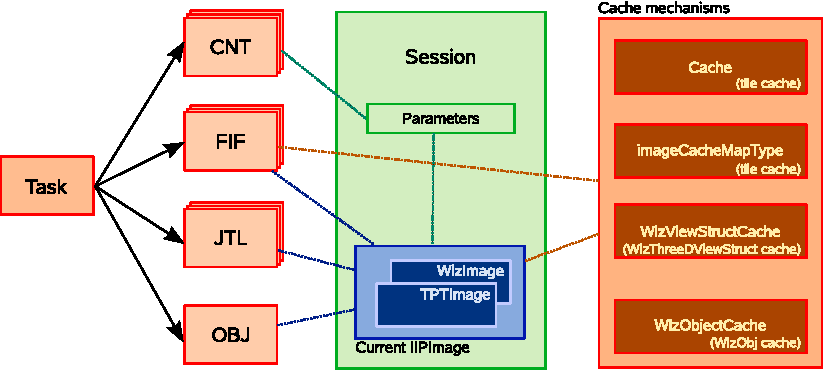
\includegraphics[width=\linewidth]{architecture}
\caption{wlziipsrv version 0.9.7 architecture}
\label{fig:architecture}
\end{figure}

Figure~\ref{fig:architecture} depicts the architecture of the WlzIIPSrv this
being inherited from the original IIPSrv and explaining both. Blocks in the
figure represent either C++ classes or structures.

The \com{Task} class is the base of all command classes that serve
independently each IIP command. Its static \texttt{factory(string type)}
method creates an instance of the appropriate class that serves the
\texttt{type} IIP command.

Figure~\ref{fig:architecture} shows some of the classes implementing the IIP
commands, all derived form the \texttt{Task}.
Four command types can be identified:
\begin{description}
\item[Parameter setting commands] such \com{CNT} and \com{ROL} pass a
parameter to the server. The parameter value is stored by the command in
the \texttt{Session} structure.
\item[Object defining commands] such \com{FIF} and \com{WLZ} receive the
file name of an object and creates the necessary structures to handle an
object.
In WlzIIPSrv, either \texttt{TPTImage} and \texttt{WlzImage} classes store
Tiled Pyramidal TIFFs and Woolz objects.
\item[Image providers] such \com{JTL}, \com{PTL} and \com{CVT} generate a
tile or a full image corresponding to the previously set parameters, stored
in the \com{Session} structure.
\item[Parameter enquiry] with \com{OBJ} command returns an parameter computed
or previously specified.
\end{description}

The \texttt{Session} structure stores all session related parameters,
including the current image object.

To reduce the computation overhead, three types of caches are used:
\begin{itemize}
\item for tiles (\texttt{RawTile}),
\item for flat images (\texttt{IIPImage})
\item for Woolz objects and view structures (\texttt{WlzObj}).
\end{itemize}

The interactions between classes, figure~\ref{fig:architecture}, are
multiple:
\begin{itemize}
\item task creates the requested command class,
\item commands set session related parameters and the current object
\item the \com{OBJ} command provides the current object parameters,
\item before loading from disc, when an operation requires access object data
      the appropriate cache structure is checked first.
      Also, when a tile is requested, if it parameters result in a cache hit
      then the cached tile is returned.
      The a Woolz view structures are cached and looked before a section is
      generated.
\end{itemize}

\subsection{IIPSrv and WlzIIPSrv beside the IIP specification}

IIP \cite[p.25]{IIP97} defines a set of mandatory and optional commands that an IIP server should implements.
The IIPSrv implements a subset of this commands, while also adds extra commands. WlzIIPSrv further extends the command set, while some of the original IIP commands are incompatible with Woolz objects.

The list of commands from Table~\ref{tab:comparision} compares command sets of the IIP specification, the IIPSrv and the WlzIIPSrv with supported (S), unsupported (N), partially implemented (P) and commands in an unknown, an undocumented or nonfunctional state (U).

\begin{table}[!hp]
\centering
\tiny{
\begin{tabular}{|c|c|c|c|}
\hline
\textbf{Command} &  \textbf{IIP spec} & \textbf{IIPSrv} & \textbf{WlzIIPSrv}\\
\hline
\com{AFN}  & S & N & N \\
\com{CIN}  & S & N & N \\
\com{CNT}  & S & S & S \\
\com{CTW}  & S & N & N \\
\com{CVT}  & S & S & S \\
\com{FIF}  & S & S & S \\
\com{FTR}  & S & N & N \\
\com{HEI}  & S & U & U \\
\com{ICC}  & S & S & U \\
\com{JTL}  & S & S & P \\
\com{OBJ}  & S & S & S \\
\com{QLT}  & S & S & S \\
\com{RAR}  & S & N & N \\
\com{RFM}  & S & N & N \\
\com{RGN}  & S & S & S \\
\com{ROI}  & S & S & S \\
\com{RST}  & S & N & N \\
\com{SDS}  & S & S & N \\
\com{TIL}  & S & S & P \\
\com{WID}  & S & U & U \\
\hline
\com{JTLS} & N & S & N \\
\com{SHD}  & N & S & U \\
\hline
\com{DST}  & N & N & S \\
\com{FXP}  & N & N & S \\
\com{FXT}  & N & N & S \\
\com{MAP}  & N & N & S \\
\com{MOD}  & N & N & S \\
\com{PAB}  & N & N & S \\
\com{PIT}  & N & N & S \\
\com{PRL}  & N & N & S \\
\com{PTL}  & N & N & S \\
\com{DPT}  & N & N & S \\
\com{RMD}  & N & N & S \\
\com{ROL}  & N & N & S \\
\com{SCL}  & N & N & S \\
\com{SEL}  & N & N & S \\
\com{UPV}  & N & N & S \\
\com{WLZ}  & N & N & S \\
\com{YAW}  & N & N & S \\
\hline
\com{Affine-transform}  & S & N & N \\
\com{App-name}          & S & U & P \\
\com{Aspect-ratio}      & S & N & N \\
\com{Author}            & S & U & N \\
\com{Basic-info}        & S & S & S \\
\com{Colorspace}        & S & S & U \\
\com{Color-twist}       & S & N & N \\
\com{Comment}           & S & U & N \\
\com{Comp-group}        & S & N & N \\
\com{Contrast-adjust}   & S & N & N \\
\com{Copyright}         & S & U & S \\
\com{Create-dtm}        & S & U & N \\
\com{Edit-time}         & S & U & N \\
\com{File-class-id}     & S & N & N \\
\com{Filtering-value}   & S & N & N \\
\com{ICC-profile}       & S & N & N \\
\com{IIP-opt-comm}      & S & S & S \\
\com{IIP-opt-obj}       & S & S & S \\
\com{IIP-server}        & S & S & S \\
\com{IIP-socket}        & S & N & N \\
\com{IIP}               & S & P & P \\
\com{Keywords}          & S & U & N \\
\com{Last-author}       & S & U & N \\
\com{Last-printed}      & S & U & N \\
\com{Last-save-dtm}     & S & U & N \\
\com{Max-size}          & S & S & S \\
\com{Property}          & S & N & N \\
\com{Render-path}       & S & N & N \\
\com{Resolution-number} & S & S & S \\
\com{Rev-number}        & S & U & N \\
\com{ROI}               & S & N & N \\
\com{Security}          & S & N & N \\
\com{Stream}            & S & N & N \\
\com{Subject}           & S & U & P \\
\com{Summary-info}      & S & U & P \\
\com{Title}             & S & U & N \\
\com{View-info}         & S & N & N \\
\hline
\com{Horizontal-views}      & N & S & U \\
\com{Tile-size}             & N & S & S \\
\com{Vertical-views}        & N & S & U \\
\hline
\com{Wlz-3d-bounding-box}   & N & N & S \\
\com{Wlz-coordinate-3D}     & N & N & S \\
\com{Wlz-distance-range}    & N & N & S \\
\com{Wlz-foreground-objects}& N & N & S \\
\com{Wlz-grey-stats}        & N & N & S \\
\com{Wlz-grey-value}        & N & N & S \\
\com{Wlz-n-components}      & N & N & S \\
\com{Wlz-sectioning-angles} & N & N & S \\
\com{Wlz-transformed-3d-bounding-box}   & N & N & S \\
\com{Wlz-transformed-coordinate-3d}        & N & N & S \\
\com{Wlz-true-voxel-size}   & N & N & S \\
\com{Wlz-volume}            & N & N & S \\
\hline
\end{tabular}
}
\caption{Command and object request support by IIP protocol,
         iipsrv0.9.7 and WlzIIPSrv. S: supported; N: not supported;
	 P: partially supported; U: unknown, an undocumented or
	 nonfunctional}
\label{tab:comparision}
\end{table}

\section{Woolz IIP Proxy}

The Woolz IIP Proxy filters and forwards IIP requests to one or more
WlzIIP servers. The requests conform the FCGI protocol. Though it was
designated to work for IIP and Woolz requests, it is generic and can
be applied to any FCGI request. Therefore, it is possible to chain
multiple proxies.

\begin{figure}[!htb]
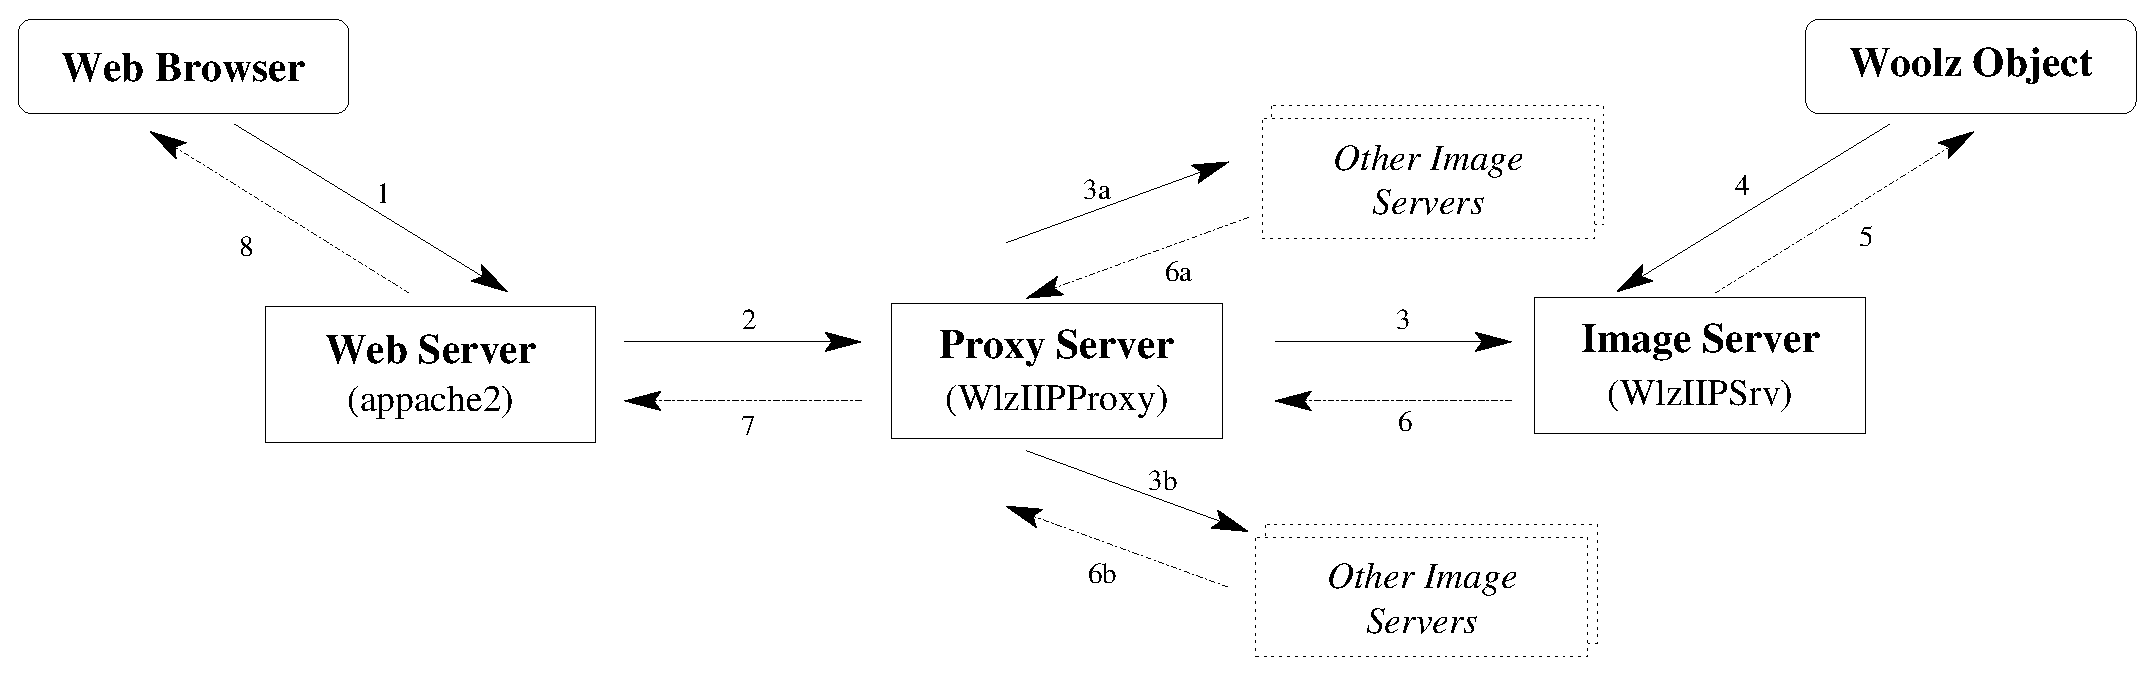
\includegraphics[width=\linewidth]{proxyarchit}
\caption{Architecture of Woolz IIP Server using a proxy server.
The proxy forwards the user web requests served first by apache
to the individual IIP Servers that have direct access to the Woolz
Object. The numbered lines show the ordering of the requests (continuous
line) and the replies (dotted lines).}
\label{fig:proxyarchit}
\end{figure}


The WlzIIPProxy is an independent program running on the proxy
server. Apache2 server forwards the FCGI request to this sever,
on a configurable port. WlzIIPSrv check the html request string
(the FCGI\_PARAMS packet QUERY\_STRING parameter) and if any
remote FCGI server definition string is a substring of the
request then request is forwarded to this server. If there is no
hit then the request is forwarded to the first FCGI remote server.
The default setup of the WlzIIPProxy architecture is shown in
figure\ref{fig:proxyarchit}


\subsection{WlzIIPProxy options}
Usage:
\begin{verbatim}
WlzIIPProxy [-p<portnumber>] [-c<conf_filename>] [-l<log_filename>]
            [-v<loglevel>] [-h]
\end{verbatim}

where the options are:
\begin{itemize}
\item -p  Port number. Default value: 123777
\item -c  Configuration file containing WLZ name to server name mapping.
          Default value: \mbox{WlzIIPProxy.conf}
\item -l  Log file name. -v with a value greater than 0 must be used.
          Default value: \mbox{/tmp/WlzIIPProxy.log}
\item -v  Log level. Default value: 0
\item -h  Help, prints usage message.
\end{itemize}

The log level is 0 to 3 with
\begin{itemize}
\item 0 -- no log,
\item 1 -- system startup, shutdown, error messages,
\item 2 -- as fcgi connection messages,
\item 3 -- as level 2 and received/sent packet types.
\end{itemize}

The configuration file has three columns for:
\begin{enumerate}
\item search string,
\item server name (or ip),
\item port number.
\end{enumerate}


\section{WlzIIPSrv installation}
\label{sec:ref:iipinstall}
\subsection{Install FastCGI}
Download and install FastCGI \cite{LIBFCGI}.
WlzIIPSrv was tested with fcgi-2.4.0 only.


\subsection{Source code}
Obtain the source files from github: 
\begin{verbatim}
https://github.com/ma-tech/WlzIIPSrv
\end{verbatim}

The following packages are also required:
\begin{verbatim}
https://github.com/ma-tech/External
https://github.com/ma-tech/Woolz
\end{verbatim}

\subsection{Compiling}
Having already built the required external libraries including the Woolz
libraries;
within the \texttt{WlzIIPSrv} root directory edit and execute the build script:
\begin{verbatim}
cp build.sh mybuild.sh
vi mybuild.sh
./mybuild.sh
\end{verbatim}

The build script can be edited, but most often this will only
need to be done to change the install prefix.
The Woolz libraries should be build with external file format support
enabled.

For doxygen documentation run \texttt{make doc}.
The documentation is generated into the \texttt{Docs} directory.

Installing implies moving the \texttt{src/wlziipsrv.fcgi} into the server's
fcgi directory:
\begin{verbatim}
cp src/wlziipsrv.fcgi /opt/apache/fcgi-bin/
\end{verbatim}
Do not forget to set read and execute access modes!

\subsection{Customisable parameters}
\label{sec:custom_param}
In addition to the IIPSrv \cite[p.25]{IIPSRV097} configuration parameters,
\texttt{WlzIIPSrv} allows with the  parameters from
Table~\ref{tab:parameters} changing the logging, caches and tile sizes.

\begin{table}[!htbp]
\centering
\begin{tabular}{|l|p{0.45\textwidth}|r|}
\hline
\textbf{Parameter}          & \textbf{Description}                        & \textbf{Default value} \\
\hline
\texttt{LOGFILE}                         & Location of log file.                                & /tmp/iipsrv.log \\
\texttt{LOGLEVEL}                        & Log level (EMERG, FATAL,                             & WARN \\
                                         & ALERT, CRIT, ERROR, WARN,                            & \\
					 & NOTICE, INFO, DEBUG).                                & \\
\texttt{FILESYSTEM\_PREFIX}              & Prefix directory for images.                         & '' \\
\texttt{MAX\_WLZOBJ\_CACHE\_SIZE}        & Maximum Woolz object cache size in MBs.              & 1024 \\
\texttt{MAX\_WLZOBJ\_CACHE\_COUNT}	 & Maximum number of Woolz object in cache.		& 100 \\
\texttt{WLZ\_TILE\_WIDTH}                & Tile width in pixels.                                & 100  \\
\texttt{WLZ\_TILE\_HEIGHT}               & Tile height in pixels.                               & 100  \\
\texttt{COMPLEX\_SELECTION}		 & Controls complex selections                          & 0 \\
                                         & with values:                                         & \\
                                         & 0 - No complex selections,                           & \\
					 & 1 - All low cost selections,                         & \\
					 & 2 - All selections.                                  & \\
\hline
\end{tabular}
\caption{WlzIIPSrv extra configuration parameters}
\label{tab:parameters}
\end{table}

The example configuration from appendix~\ref{sec:httpconf} defines a view
structure cache with 200 structures, a 1500MB Woolz object cache
and $100\times100$ tile size.

\section{WlzIIPProxy installation}
\label{sec:fcgi:install}

\begin{itemize}
\item Download and compile / install FastCGI \cite{LIBFCGI}.

\item Get WlzIIPProxy source code from the CVS repository:
\begin{verbatim}
cvs checkout -P src/Applications/WlzIIPProxy
\end{verbatim}

\item Configure and compile WlzIIPProxy:
Run from the \texttt{WlzIIPSrv} root directory
\begin{verbatim}
aclocal; autoheader; automake; autoconf; ./configure; make
\end{verbatim}


\item Run WlzIIPProxy on the desired port and using the configuration file.
\begin{verbatim}
WlzIIPProxy -p <portnumber> -c <config_file>
\end{verbatim}

\item Configure apache2 on the web server:
\begin{enumerate}
  \item install mod\_fastcgi (you might need to reinstall apache2)
  \textbf{Note:} the mod\_fcgi module, provided in SUSE 10.3 can not make
  remote FCGI request therefore is not compatible with WlzIIPSrv.
  mod\_fastcgi must be used.
  \item add to httpd.conf (/opt/apache/conf//httpd.conf):
\end{enumerate}
\begin{verbatim}
  FastCgiExternalServer <virtual_path_to_fcgi> -host <hostname>:<portnumber>
\end{verbatim}
\end{itemize}

\section{Acknowledgement}

We gratefully acknowledge the support from NIH under grant \#1R01MH070370-01A2.

\appendix

\section{fcgi configuration}
\label{sec:httpconf}
An example of the apache2 configuration
(\texttt{/opt/apache/conf/httpd.conf})
is\footnote{This configuration file is compatible with mod\_fcgi.
For mod\_fastcgi alternative format must be used (see IIPSrv web-page).}

\begin{verbatim}
# Create a directory for the iipsrv binary
ScriptAlias /fcgi-bin/ "/opt/apache/fcgi-bin/"

# Set the options on that directory
<Directory "/opt/apache/fcgi-bin">
   AllowOverride None
   Options None
   Order allow,deny
   Allow from all
   # Set the module handler
   AddHandler fcgid-script .fcgi
</Directory>

# Initialise the FCGI server and set some default values
FastCgiServer /opt/apache/fcgi-bin/wlziipsrv.fcgi \
-initial-env LOGFILE=/opt/apache/logs/wlziipsrv.log \
-initial-env LOGLEVEL=WARN \
-initial-env JPEG_QUALITY=50 \
-initial-env FILESYSTEM_PREFIX=/export/images \
-initial-env MAX_CVT=3000 \
-initial-env MAX_WLZOBJ_CACHE_COUNT=100 \
-initial-env MAX_WLZOBJ_CACHE_SIZE=4000 \
-initial-env WLZ_TILE_WIDTH=100 \
-initial-env WLZ_TILE_HEIGHT=100 \
-initial-env COMPLEX_SELECTION=0
\end{verbatim}

\bibliographystyle{apalike}
\bibliography{biblio}

\end{document}
